\documentclass{article}\usepackage[]{graphicx}\usepackage[]{color}
% maxwidth is the original width if it is less than linewidth
% otherwise use linewidth (to make sure the graphics do not exceed the margin)
\makeatletter
\def\maxwidth{ %
  \ifdim\Gin@nat@width>\linewidth
    \linewidth
  \else
    \Gin@nat@width
  \fi
}
\makeatother

\definecolor{fgcolor}{rgb}{0.345, 0.345, 0.345}
\newcommand{\hlnum}[1]{\textcolor[rgb]{0.686,0.059,0.569}{#1}}%
\newcommand{\hlstr}[1]{\textcolor[rgb]{0.192,0.494,0.8}{#1}}%
\newcommand{\hlcom}[1]{\textcolor[rgb]{0.678,0.584,0.686}{\textit{#1}}}%
\newcommand{\hlopt}[1]{\textcolor[rgb]{0,0,0}{#1}}%
\newcommand{\hlstd}[1]{\textcolor[rgb]{0.345,0.345,0.345}{#1}}%
\newcommand{\hlkwa}[1]{\textcolor[rgb]{0.161,0.373,0.58}{\textbf{#1}}}%
\newcommand{\hlkwb}[1]{\textcolor[rgb]{0.69,0.353,0.396}{#1}}%
\newcommand{\hlkwc}[1]{\textcolor[rgb]{0.333,0.667,0.333}{#1}}%
\newcommand{\hlkwd}[1]{\textcolor[rgb]{0.737,0.353,0.396}{\textbf{#1}}}%
\let\hlipl\hlkwb

\usepackage{framed}
\makeatletter
\newenvironment{kframe}{%
 \def\at@end@of@kframe{}%
 \ifinner\ifhmode%
  \def\at@end@of@kframe{\end{minipage}}%
  \begin{minipage}{\columnwidth}%
 \fi\fi%
 \def\FrameCommand##1{\hskip\@totalleftmargin \hskip-\fboxsep
 \colorbox{shadecolor}{##1}\hskip-\fboxsep
     % There is no \\@totalrightmargin, so:
     \hskip-\linewidth \hskip-\@totalleftmargin \hskip\columnwidth}%
 \MakeFramed {\advance\hsize-\width
   \@totalleftmargin\z@ \linewidth\hsize
   \@setminipage}}%
 {\par\unskip\endMakeFramed%
 \at@end@of@kframe}
\makeatother

\definecolor{shadecolor}{rgb}{.97, .97, .97}
\definecolor{messagecolor}{rgb}{0, 0, 0}
\definecolor{warningcolor}{rgb}{1, 0, 1}
\definecolor{errorcolor}{rgb}{1, 0, 0}
\newenvironment{knitrout}{}{} % an empty environment to be redefined in TeX

\usepackage{alltt}
\usepackage{Sweave}
\usepackage{float}
\usepackage{graphicx}
\usepackage{tabularx}
\usepackage{siunitx}
\usepackage{amssymb} % for math symbols
\usepackage{amsmath} % for aligning equations
\usepackage{textcomp}
\usepackage{mdframed}
\usepackage{natbib}
\bibliographystyle{..//references/styles/besjournals.bst}
\usepackage[small]{caption}
\setlength{\captionmargin}{30pt}
\setlength{\abovecaptionskip}{0pt}
\setlength{\belowcaptionskip}{10pt}
\topmargin -1.5cm        
\oddsidemargin -0.04cm   
\evensidemargin -0.04cm
\textwidth 16.59cm
\textheight 21.94cm 
%\pagestyle{empty} %comment if want page numbers
\parskip 7.2pt
\renewcommand{\baselinestretch}{1.5}
\parindent 0pt
%\usepackage{lineno}
%\linenumbers

%cross referencing:
\usepackage{xr}
\usepackage{xr-hyper}
\externaldocument{/Users/CatherineChamberlain/Documents/git/chillfreeze/docs/chillfrz_supp}

\newmdenv[
  topline=true,
  bottomline=true,
  skipabove=\topsep,
  skipbelow=\topsep
]{siderules}
\IfFileExists{upquote.sty}{\usepackage{upquote}}{}
\begin{document}

\noindent \textbf{\Large{False spring damage on temperate tree seedlings is amplified with winter warming}}

\noindent Authors:\\
C. J. Chamberlain $^{1,2}$, K. Woodruff $^{1}$ \& E. M. Wolkovich $^{1,2,3}$
\vspace{2ex}\\
\emph{Author affiliations:}\\
$^{1}$Arnold Arboretum of Harvard University, 1300 Centre Street, Boston, Massachusetts, USA; \\
$^{2}$Organismic \& Evolutionary Biology, Harvard University, 26 Oxford Street, Cambridge, Massachusetts, USA; \\
$^{3}$Forest \& Conservation Sciences, Faculty of Forestry, University of British Columbia, 2424 Main Mall, Vancouver, BC V6T 1Z4\\
\vspace{2ex}
$^*$Corresponding author: 248.953.0189; cchamberlain@g.harvard.edu\\

\renewcommand{\thetable}{\arabic{table}}
\renewcommand{\thefigure}{\arabic{figure}}
\renewcommand{\labelitemi}{$-$}
\setkeys{Gin}{width=0.8\textwidth}

%%%%%%%%%%%%%%%%%%%%%%%%%%%%%%%%%%%%%%%%%%%%%%%
%%%%%%%%%%%%%%%%%%%%%%%%%%%%%%%%%%%%%%%%%%%%%%%


\section*{Introduction}
\begin{enumerate}
\item The timing of spring in temperate deciduous forests shapes plant and animal communities and influences ecosystem services from agriculture to carbon sequestration to forest management. 
  \begin{enumerate} 
  \item With warming temperatures in the Northern Hemisphere, spring phenology (i.e., budburst and leafout, which  are strongly cued by temperature) is advancing causing longer growing seasons \citep{Chuine2001} and reshaping these services.  
  \item In one major example, advancing spring phenology has lead to increased carbon uptake across temperate forests, which are essential carbon sinks that combat the negative effects of climate change \citep{Keenan2014}.
  \item But climate change has other important effects that could cause declines in these services: specifically cold snaps during the spring and reduced cool temperatures in the winter. 
  \end{enumerate}
  
\item And though the Northern Hemisphere is getting warmer, climate change is affecting general temperature trends but extreme weather events (e.g., polar vortexes) are still occurring. 
  \begin{enumerate}
  \item These weather events can in turn have big impacts on plant development each spring. 
  \item One such event is known as a `false spring', which is when temperatures drop below freezing \citep[][i.e., below -2.2$^{\circ}$C]{Schwartz2002} after budburst has initiated.
  \item Damage from false spring events can have cascading effects to pollinators \citep{Boggs2012, Pardee2017}, nutrient cycling and carbon uptake as well as forest recruitment \citep{Hufkens2012, Klosterman2018, Richardson2013}.
  \end{enumerate}

\item Further false springs can increase the chance of additional false springs within a growing season by extending the period that plants are most at risk---the time between budburst and leafout (what we refer to as the `duration of vegetative risk'). 
  \begin{enumerate}
  \item Observational studies suggest plants take longer to re-flush leaves after a false spring--up to 38 days \citep{Augspurger2009, Augspurger2013, Gu2008, Menzel2015}, which could lead to additional false springs in a season \citep{Augspurger2009}.
  \item False springs are predicted to increase in certain regions as climate change progresses, thus understanding the impacts of false springs on forests is essential for forest management strategies and climate forecasting \citep{OBrien2019}.
  \end{enumerate}
  
\item Warmer winters may also play a critical role in the future of forests as they directly impact one of the  major cues plants use to time budburst: over-winter cold temperatures (chilling), (in addition to warming spring temperatures (forcing) and longer daylengths).
  \begin{enumerate}
  \item Many temperate plants have evolved chilling requirements to avoid leafout during warm snaps in the middle of the winter, but with climate change chilling requirements may not be met. 
  \item  If chilling is not met, plants may leaf out much slower or incompletely, which can in turn affect freeze tolerance. 
  \item Thus, understanding the interplay of warming winters and false spring risk is critical to predict how temperate forests will change in the future.
  \end{enumerate} 
  
  
\item This interaction between winter chilling and false springs may vary across species within a community, as species have likely evolved along a trade-off of risking spring frosts for early access to resources.
  \begin{enumerate}
  \item Ideally, individuals would evolve to require high levels of chilling to delay budburst and ultimately diminish false spring risk but competition for nutrients, water and light resources in the early spring pushes individuals to leafout earlier. 
  \item Young trees and understory species generally initiate budburst before the canopy trees to benefit from higher light levels \citep {Augspurger2008, Vitasse2013}, which potentially puts these species and individuals at higher risk of freeze damage \citep{Vitasse2014}.
  \item Thus, successful forest recruitment requires seedlings and saplings to minimize false spring risk while maximizing growth.
   \end{enumerate}
 

\item The combination of species-level differences in responses to false springs and chilling and climate change could reshape the temporal assembly of forest communities. 
  \begin{enumerate}
  \item Species typically leafout in a similar sequence, with understory species leafing out earlier and higher canopy trees leafing out last but many studies are predicting substantial shifts in chronological order and reassembly of species' leafout with climate change \citep{Roberts2015, Laube2014}.
  \item As warming alters winter temperatures and false spring prevalence, phenological cues and their interactions are anticipated to change, which could greatly alter competition and recruitment among forest species for early season resources and ultimately impact species diversity and carbon uptake in temperate forests.
  \end{enumerate}
  
\item Here, we assessed the effects of over-winter chilling length and false springs on seedling phenology and growth across eight temperate tree and shrub species. 
  \begin{enumerate}
  \item Individuals were exposed to different levels of over-winter chilling and then half of the individuals were exposed to a false spring event. 
  \item Individuals were observed for the remainder of the growing season to ask: (1) How does the accumulation of over-winter chilling hours and (2) how do false spring events impact phenology, physical leaf characteristics and growth?
  \end{enumerate}
\end{enumerate}
  

\section*{Methods}
\subsection*{Plant Selection and Material}
\begin{enumerate}
\item We used 8 temperate woody plant tree and shrub species with varying phenologies, that were not used as crops or ornamental species: \textit{Acer saccharinum} L., \textit{Alnus incana rugosa} L., \textit{Betula papyrifera} Marsh., \textit{Betula populifolia} Marsh., \textit{Cornus racemosa} Lam., \textit{Salix purpurea} L., \textit{Sorbus americana} Marsh., and \textit{Viburnum dentatum} L. Two additional species---\textit{Fagus grandifolia} and \textit{Nyssa sylvatica}---were also originally included in the experimental design, but were not delivered in a usable condition and thus could not be used in the experiment.
  \begin{enumerate}
  \item We received 48 dormant bare root seedlings---each measuring 6-12 inches---for each species from Cold Stream Farm LLC (Freesoil, MI; 44$^{\circ}$6' N -86$^{\circ}$12' W) for a total of 384 individuals.
  \item Upon receipt, plants were potted in POT INFO AND SOIL INFO HERE!! and placed in growth chambers at the Weld Hill Research Building of the Arnold Arboretum (Boston, MA; 42$^{\circ}$17' N -71$^{\circ}$8' W) at 4$^{\circ}$C to maintain dormancy.
  \item After all individuals had leafed out, all seedlings were up-potted to new pots (NEW POT SIZE HERE) and given fertilizer (FERTILIZER INFO HERE).
  \end{enumerate}
\end{enumerate}
\subsection*{Growth Chamber and Greenhouse Conditions}
\begin{enumerate}
\item Individuals were randomly selected and placed in six experimental treatments: 4 weeks of chilling at 4$^{\circ}$C x no false spring, 4 weeks of chilling at 4$^{\circ}$C x false spring, 6 weeks of chilling at 4$^{\circ}$C x no false spring, 6 weeks of chilling at 4$^{\circ}$C x false spring,
8 weeks of chilling at 4$^{\circ}$C x no false spring, 8 weeks of chilling at 4$^{\circ}$C x false spring.
  \begin{enumerate}
  \item While individuals were in the growth chamber under chilling conditions, photoperiod was maintained at eight hour days.
  \item Lighting within the chambers was provided through a combination of T5HO fluorescent lamps with halogen incandescent bulbs at roughly 250 $\mu mol/m^{2}/s$.
  \item Individuals were rotated within and among growth chambers every two weeks to eliminate possible growth chamber effects.
  \end{enumerate}
\item Once chilling was completed, individuals were moved to a greenhouse with mean daytime temperature of 15$^{\circ}$C and a mean nighttime temperature of 10$^{\circ}$C.
  \begin{enumerate}
  \item Photoperiod was set to 12 hour days throughout the spring until all individuals reached full leaf expansion.
  \item After all individuals of all species reached full leaf expansion, greenhouse temperatures and photoperiods were kept ambient (see Supplemental Materials for more information). 
  \end{enumerate}
\end{enumerate}
\subsection*{Phenology and False Spring Treatment}
\begin{enumerate}
\item Phenology observations were taken every 2-3 days through full leaf expansion and then recorded weekly over the summer. 
  \begin{enumerate}
  \item Budburst was denoted as BBCH stage 07, which is `beginning of sprouting or bud breaking' and monitored until full leaf expansion (BBCH stage 19) in order to evaluate the duration of vegetative risk \citep{Chamberlain2019} for each individual \citep{Finn2007}.
  \item Individuals in the `false spring treatment' were placed in a growth chamber set to mimic a false spring event during budburst, defined as once at least 50\% of the buds were at BBCH stage 07 but the individual had not yet reached BBCH stage 19 (that is, each individual was exposed to a false spring based on its individual phenological timing). 
  \item Individuals receiving the false spring treatment were placed in a growth chamber for 14 hours, starting at 6pm. 
  \item Temperatures in the growth chamber were ramped down over 14 hours (Figure \ref{fig:gccond}).
  \item After 8am the following day, individuals were collected at placed back in the greenhouse with all of the other plants. 
  \item Once all individuals reached full leaf expansion (BBCH stage 19), we made weekly phenology observations until August 1st and then we made observations every 2-3 days again to monitor fall phenology.
  \item Individuals were monitored until complete budset, at which point they were harvested for biomass measurements.
  \end{enumerate}
\end{enumerate}
\subsection*{Growth measurements}
\begin{enumerate}
\item Growth was closely measured throughout the entirety of the experiment. 
  \begin{enumerate}
  \item Height was measured three times throughout the growing season: the day an individual reached full leaf expansion, 60 days after full leaf out and when an individual reached complete budset. 
  \item We measured the chlorophyll content of four leaves on each individual 60 days after full leaf out using an atLEAF CHL PLUS Chlorophyll meter.
  \item The average chlorophyll content was calculated and then converted to mg/cm\textsuperscript{2} using the atLEAF CHL PLUS conversion tool.
  \item We measured leaf thickness using a Shars Digital Micrometer (scale works to 0.001mm) and leaf toughness in Newtons using a Shimpo Digital Force Gauge on two leaves for each individual.
  \item Additionally, we visually monitored damage to the shoot apical meristem, which consisted of complete damage or disruption of growth in the main stem and resulted in early dormancy induction or reliance on lateral shoot growth.
  \item Finally, belowground and aboveground biomass were harvested after an individual reached complete budset to include leaves in our biomass calculations. 
  \item Belowground and aboveground plant material were separated and then put in a Shel Lab Forced Air Oven at 60$^{\circ}$C for at least 4 days. 
  \end{enumerate}
\end{enumerate}
\subsection*{Data analysis}
\begin{enumerate}
\item Using Bayesian hierarchical models with the brms package \citep{brms}, version 2.3.1,  in R \citep{R}, version 3.3.1, we estimated the effects of chilling duration, false spring treatment and all two-way interactions as predictors on: (1) duration of vegetative risk, (2) growing season length, (3) total growth in centimeters, (4) chlorophyll content, (5) leaf thickness, (6) leaf toughness, (7) shoot apical meristem damage and (8) total biomass. % CUT FOR NOW: and (9) belowground to aboveground biomass ratio. 
  \begin{enumerate} 
  \item Species were modeled hierarchically as grouping factors, which generates an estimate and posterior distribution of the overall response across the eight species used in our experiment.
  \item We ran four chains, each with 2 500 warm-up iterations and 4 000 sampling iterations for a total of 6 000 posterior samples for each predictor for each model using weakly informative priors. 
  \item Increasing priors three-fold did not impact our results.
  \item We evaluated our model performance based on $\hat{R}$ values that were close to one and did not include models with divergent transitions in our results. 
  \item We also evaluated high $n_{eff}$ (4000 for most parameters, but as low as 1400 for a couple of parameters in the shoot apical meristem model). 
  \item We additionally assessed chain convergence and posterior predictive checks visually \citep{BDA}.
  \end{enumerate}
\end{enumerate}

\section*{Results}
\begin{enumerate}
\item False springs and chilling durations both impacted individual phenology. 
  \begin{enumerate}
  \item Individuals exposed to the false spring treatment had longer durations of vegetative risk for the four weeks and slightly for the six weeks of chilling cohort (2.97 $\pm$ 0.79 days and 1.53 $\pm$ 1.14 days, respectively; Figure \ref{fig:muphen}\textbf{a} and Table \ref{tab:suppmoddvr}).
  \item Longer chilling treatments reduced the duration of vegetative risk, especially in the eight weeks of chilling cohort (-2.67 $\pm$ 1.14 days; Figure \ref{fig:muphen}\textbf{a} and Table \ref{tab:suppmoddvr}).
  \item Additionally, as seen in a simple linear model (Table \ref{tab:simpbb}), increases in chilling duration advanced day of budburst by -2.79 $\pm$ 1.74 days for six weeks of chilling and by -7.63 $\pm$ 1.76 days for eight weeks of chilling.
  \end{enumerate}
  
\item Effects on the duration of vegetative risk from false spring (longer) and from increased chilling (shorter) were generally additive, resulting in no major changes in the durations of vegetative risk for individuals exposed to a false spring that received eight weeks of chilling (0.92 $\pm$ 1.08 days, Figure \ref{fig:muphen}\textbf{a} and Table \ref{tab:suppmoddvr}). 
  \begin{enumerate}
  \item With increases in chilling duration, the growing season length decreased for individuals exposed to six and eight weeks of chilling (2.48 $\pm$ 4.87 days for six weeks and -9.66 $\pm$ 5 days for eight weeks; Figure \ref{fig:muphen}\textbf{b} and Table \ref{tab:suppmodgs}).
  \end{enumerate}
  
\item False springs impacted growth habit but not total biomass. 
  \begin{enumerate}
  \item Across all chilling treatments, especially for the four and eight week cohorts, individuals exposed to false springs experienced more damage to the shoot apical meristem (51.7\% increase in probability of damage under false spring treatment or 2.07 $\pm$ 0.97 for four weeks, -5.2\% or a 1.33 $\pm$ 1.42 for six weeks and 7\% or a 2.17 $\pm$ 1.31 for eight weeks; Figure \ref{fig:mugrowth}\textbf{a} and Table \ref{tab:suppmodmeri}) .
  \item Shoot growth over the growing season increased with eight weeks of chilling (11 $\pm$ 4.01 cm) except growth was not affected under false spring conditions (4.73 $\pm$ 5.49 cm; Figure \ref{fig:muheight} and Table \ref{tab:suppmodht})). %CJC 17 July 2020: should I move this figure to the main doc and then move the totbiomass figure to the supp? 
  \item Individuals exposed to false spring conditions had slightly lower total biomasses when they were exposed to only four weeks of chilling (-3.45 $\pm$ 2.78 g) but there was very little change in total biomass under false spring conditions compared to the control for both the six weeks of chilling cohort (-3.62 $\pm$ 4.04 g) and the eight weeks of chilling cohort (2.88 $\pm$ 3.04 g; Figure \ref{fig:mugrowth}\textbf{b} and Table \ref{tab:suppmodtotbio})).
  \end{enumerate}
  
\item False springs affected physical leaf traits.
  \begin{enumerate}
  \item Leaf chlorophyll content decreased under false spring conditions with increases in chilling, especially with eight weeks of chilling (-1.45 $\pm$ 1.16 mg/cm\textsuperscript{2} for six weeks and -2.03 $\pm$ 1.07 mg/cm\textsuperscript{2} for eight weeks; Figure \ref{fig:muchl} and Table \ref{tab:suppmodchl}).
  \item Leaf toughness decreased across all chilling treatments under false spring conditions (-0.05 $\pm$ 0.02 N for four weeks of chilling, -0.09 $\pm$ 0.03 N for six weeks of chilling and -0.08 $\pm$ 0.03 N for eight weeks of chilling; Figure \ref{fig:muleaf}\textbf{a} and Table \ref{tab:suppmodtough}).
  \item Additionally, leaf thickness decreased across four and eight week chilling durations under false spring conditions, but there was little change for the six weeks of chilling cohort (-8.9 $\pm$ 3.74 $\mu$m for four weeks of chilling, -3.5 $\pm$ 5.31 $\mu$m for six weeks of chilling and -15.78 $\pm$ 5.25 $\mu$m for eight weeks of chilling; Figure \ref{fig:muleaf}\textbf{b} and Table \ref{tab:suppmodthick}).
  \end{enumerate}
  
  
\item False springs and chilling duration treatments resulted in only some species-level differences.
 \begin{enumerate}
  \item Duration of vegetative risk decreased for most species with long chilling durations (i.e., the eight week cohort), except for \textit{Salix purpurea}, which experienced longer durations of vegetative risk with longer chilling durations (Figure \ref{fig:muphen}\textbf{a}). 
  \item All species experienced meristem damage under false spring conditions except for \textit{Betula populifolia} and \textit{Sorbus americana}.
  \item Additionally, \textit{Viburnum dentatum} experienced meristem damage under all treatments (Figure \ref{fig:mugrowth}\textbf{a}). 
  \item There was a lot of species-level variation with leaf thickness under the longer chilling durations, with \textit{Sorbus americana} and \textit{Viburnum dentatum} having thicker leaves with increases in chilling (Figure \ref{fig:muleaf}\textbf{b}). 
  \end{enumerate}
  
\item Despite large treatment effects on phenology, we found no major effects on phenological rank within the community.
  \begin{enumerate}
  \item Order of leafout timing was consistent across all treatments, with \textit{Salix purpurea} always being first to leafout, followed by \textit{Betula papyrifera}, \textit{B. populifolia} and \textit{Cornus racemosa} and finally by \textit{Alnus rugosa}, \textit{Sorbus americana}, \textit{Viburnum dentatum} and \textit{Acer saccharinum} (Figure \ref{fig:rank}).
  \item \textit{Viburnum dentatum} was the only species to change rank across treatments, though it consistently was grouped with the later-leafout group of species.
  \item Order of budset timing was also consistent across all treatments, with \textit{Cornus racemosa} and \textit{Sorbus americana} being first to set bud, followed by \textit{Betula papyrifera} and \textit{Acer saccharinum} and finally by \textit{Viburnum dentatum}, \textit{B. populifolia}, \textit{Salix purpurea} and \textit{Alnus rugosa} (Figure \ref{fig:bsetrank}).
  \item \textit{Acer saccharinum} was the only species to change rank across treatments, though it consistently was grouped with \textit{Betula papyrifera} and \textit{Viburnum dentatum}.
  \end{enumerate}
\end{enumerate}

\section*{Discussion} 
\begin{enumerate}
\item Our experiment replicated the major features of false springs---causing plant damage---and chilling---advancing spring phenology, allowing us to examine the cascading consequences of these two interactive effects of climate change across eight deciduous forest tree species. Our results showed these effects altered multiple aspects of plant phenology, plant growth and leaf traits. Importantly, we found false springs and chilling have opposing additive effects on the duration of vegetative risk, suggesting the combination of increased false springs and warmer winters could be especially detrimental.

\subsection*{False springs and chilling interactively determine risk and damage}
\item Chilling length greatly influences spring phenology during the critical budburst to leafout phases, and thus can compensate for the detrimental effects of false springs on phenology.
  \begin{enumerate}
  \item With false springs increasing the duration of vegetative risk, the risk of multiple false springs occuring in one season also increases. 
  \item But chilling can compensate for this increase in duration of vegetative risk: with increased chilling, the duration of vegetative risk does not increase under false spring conditions.
  \item This suggests chilling is more important for seedlings in terms of exposure to multiple false springs.
  \item With climate change and warming temperatures, over-winter chilling is anticipated to decrease and false springs are predicted to increase in certain regions.
  \item This combination could greatly impact plant performance, survival and shape species distributions, ultimately affecting crucial processes such as carbon uptake and nutrient cycling.
  \end{enumerate}
  
\item False springs impact seedling growth, regardless of chilling duration.
  \begin{enumerate}
  \item Past studies suggest early-budburst species can withstand lower temperature thresholds \citep{Lenz2013, Muffler2016, Zohner2020}, our results suggest false springs consistently impair shoot apical meristem growth, regardless of phenological order. 
  \item Damage to the shoot apical meristem can lead to reliance on lateral shoot growth, rendering inefficient growth patterns and, if damage is significant within a stand, it can lead to declines in recruitment \citep{Rhodes2018}. 
  \item Though overall height increased with more over-winter chilling, false springs impacted all individuals similarly across all chilling treatments, thus further emphasizing the detrimental effects of meristem damage. 
  \end{enumerate}
  
\item False springs greatly impact the physical characteristics of the leaf.
  \begin{enumerate}
  \item With chlorophyll content, leaf toughness and leaf thickness decreasing, the quality of the leaf dwindles.
  \item This reduction in quality could subsequently lead to an increase in herbivory risk \citep{Onoda2011}.
  \item We found that increased chilling levels actually decreased leaf toughness and decreased chlorophyll content under false spring conditions.
  \item Further studies that assess the secondary compounds and total phenolic content \citep{Ayres1993, Webber2016} as well as photosynthetic rate of the leaves exposed to false springs after varying durations of chilling, are needed to better understand the level of herbivory risk and the overall quality of the leaf.
  \end{enumerate}

\subsection*{False springs and chilling do not reshape temporal assembly}
\item Climate model projections and no chilling treatments in growth chamber studies predict substantial shifts in species leafout order under climate change conditions \citep{Roberts2015, Laube2014}, other studies using long-term phenology observations suggest leafout phenology order is consistent across years \citep{Wesolowski2006}.
  \begin{enumerate}
  \item We are not seeing major shifts in species leafout order---thus consistent with observational studies \citep{Wesolowski2006}---except for in \textit{Viburnum dentatum}, which still leafs out within the later cohort of species across all treatments.
  \item Therefore, we do not predict major reassembly of forest communities due to winter warming or false spring incidence. 
  \item As was evident from a growth chamber study, most treatments did not render substantial phenological reordering, except under no chilling treatments \citep{Laube2014}. Our results differ from projections---and this no chilling treatment---and this is likely due to greater decreases in over-winter chilling under future climate conditions, which was not fully captured in our experimental design.
    \end{enumerate}
    
\item Phenological rank remains consistent across all false spring and chilling treatments, as long as all individuals are affected equally.
  \begin{enumerate}
  \item In nature, not all of our study species are at equal risk of false springs, with early-budburst species (e.g., \textit{Salix americana} or \textit{Betula papyrifera}) generally more at risk than later-budburst species (e.g., \textit{Acer saccharinum} or \textit{Viburnum dentatum}). 
  \item This suggests we could in fact expect climate change to reshape forest communities, but it may not come from temporal assembly directly, but rather from the damage and leaf trait impacts of false springs and decrease in chilling duration.
  \end{enumerate}

\item Understanding the impacts of false springs coupled with reduced over-winter chilling is essential for forecasting.
  \begin{enumerate}
  \item Our findings have large implications for forest recruitment.
  \item With over-winter chilling decreasing with climate change, seedlings are more at risk of sustaining damage from false spring events. 
  \item Understanding recruitment and inter- and intraspecific competition with false springs is crucial. 
  \item If individuals that initiate budburst earlier are more at risk of false spring exposure, this could lead to dieback of early-budbursting species in temperate forests with climate change. 
  \item Climate change could greatly impact early-budburst species as these individuals will likely see increases in durations of vegative risk with the dual effects of lower chilling and heightened false spring risk. 
  \item By integrating the additive and adverse effects of decreasing over-winter chilling and increasing false spring risk, we can better predict shifts in forest communities and recruitment under climate change. 
  \end{enumerate}
\end{enumerate}




\bibliography{..//references/chillfreeze.bib}

\section*{Tables and Figures}

{\begin{figure} [H]
  -\begin{center}
  -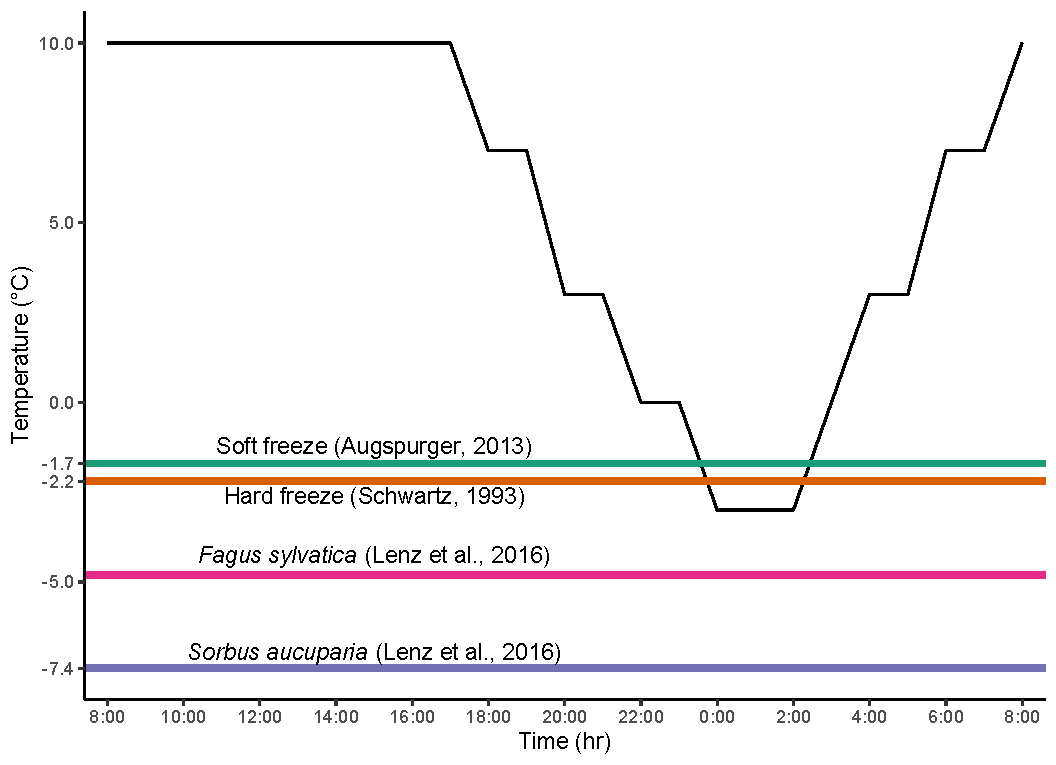
\includegraphics[width=12cm]{..//analyses/figures/growthchamber.pdf}
  -\caption{False spring treament temperature regime in the growth chamber}\label{fig:gccond}
  -\end{center}
  -\end{figure}}

  {\begin{figure} [H]
  -\begin{center}
  -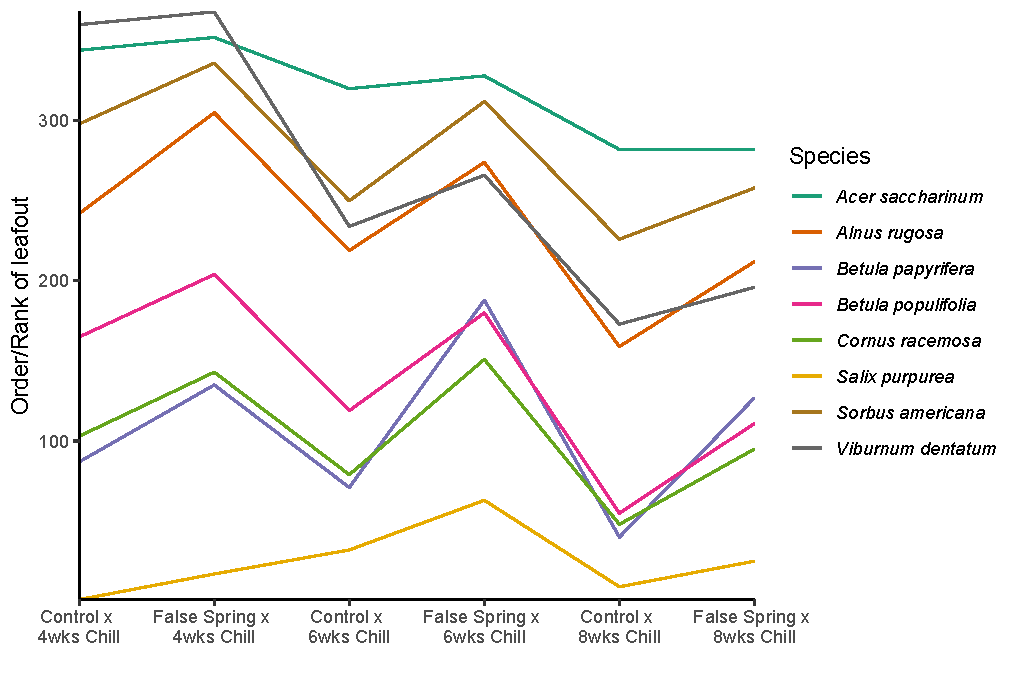
\includegraphics[width=12cm]{..//analyses/figures/leafoutorder_byrank.pdf} 
  -\caption{Understanding rank order of leafout across all species using (a) mean trends and (b) raw estimates. }\label{fig:rank}
  -\end{center}
  -\end{figure}}
  
  {\begin{figure} [H]
  -\begin{center}
  -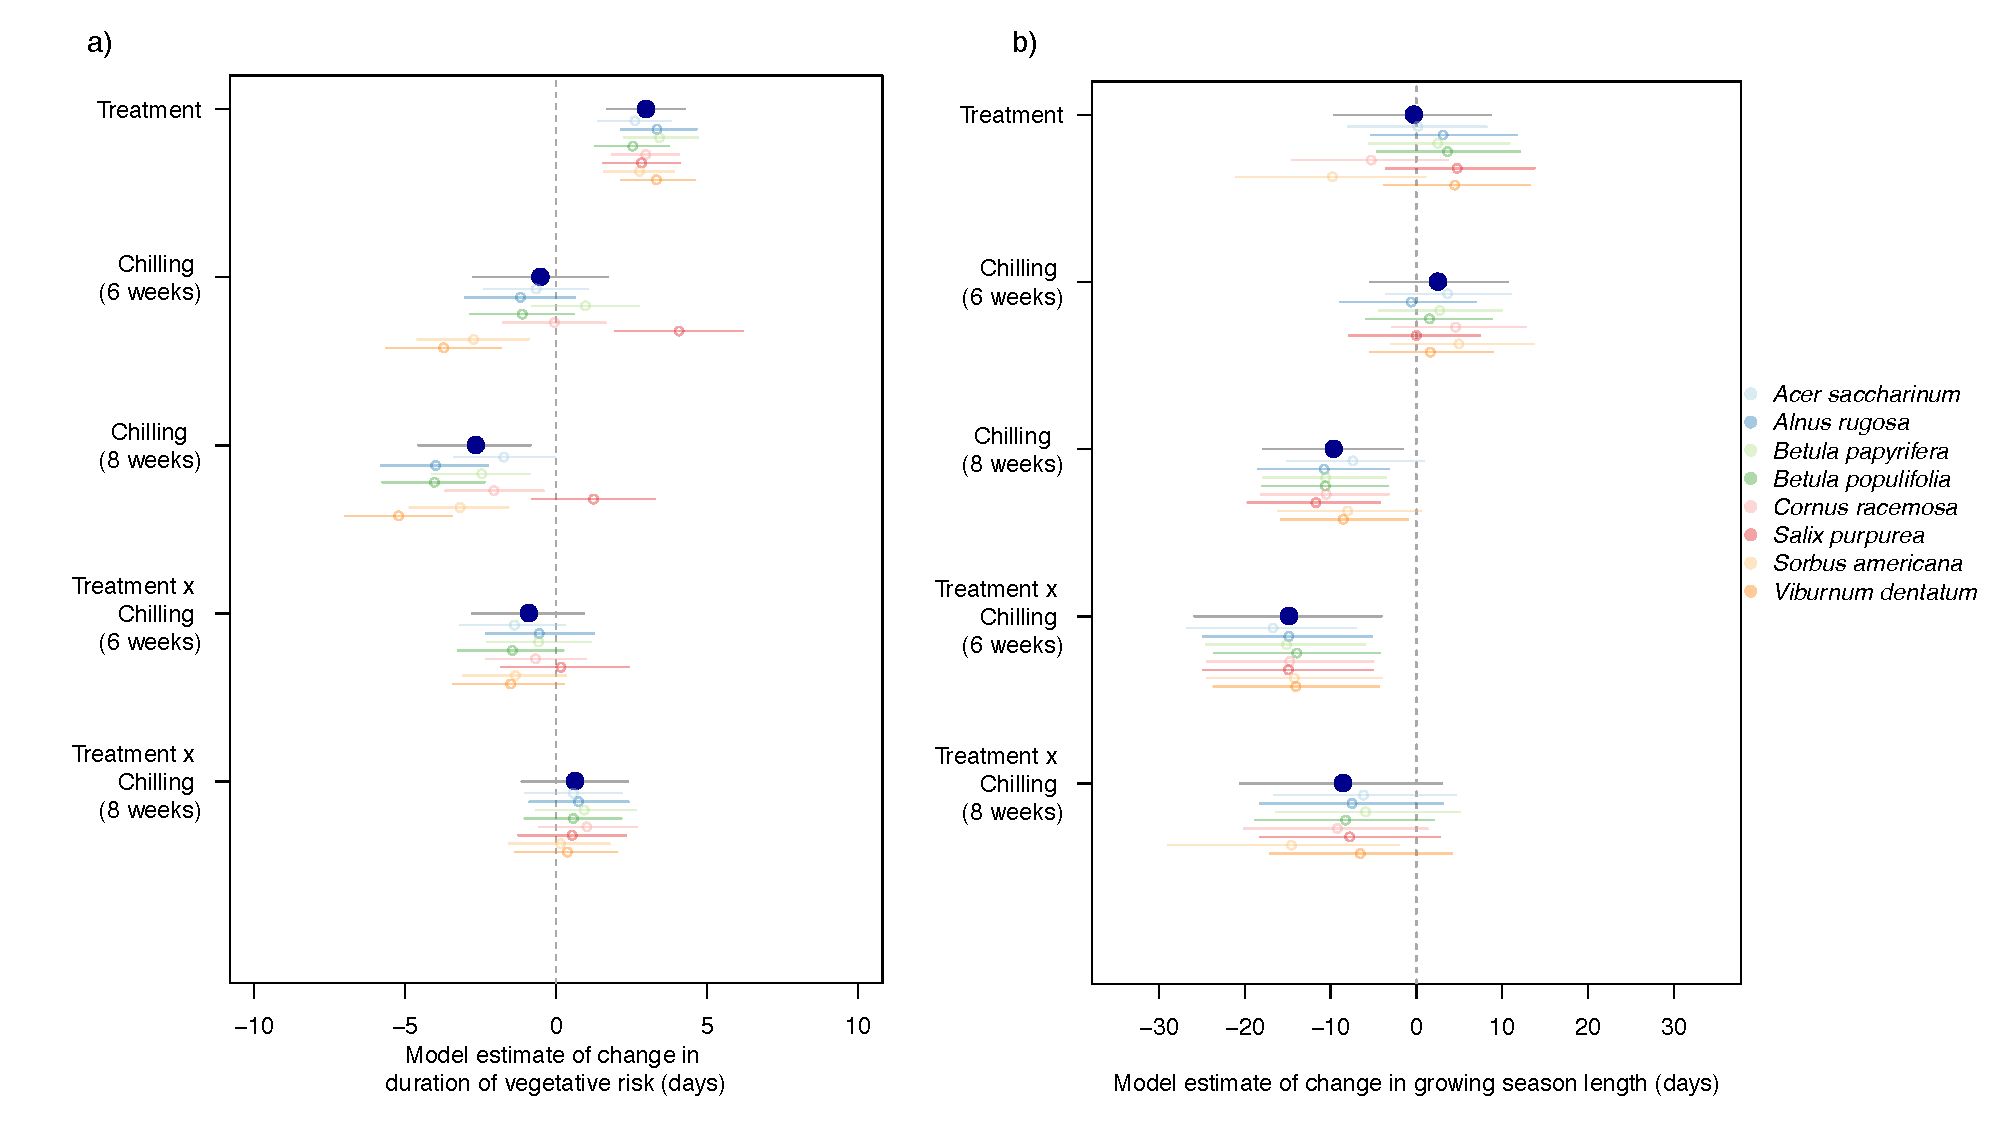
\includegraphics[width=18cm]{..//analyses/figures/mu_phen90.pdf} 
  -\caption{Effects of false spring treatment, six weeks of chilling and eight weeks of chilling on a) duration of vegetative risk and b) growing season length. Dots and lines show means and 90\% uncertainty intervals.}\label{fig:muphen}
  -\end{center}
  -\end{figure}}
  
  {\begin{figure} [H]
  -\begin{center}
  -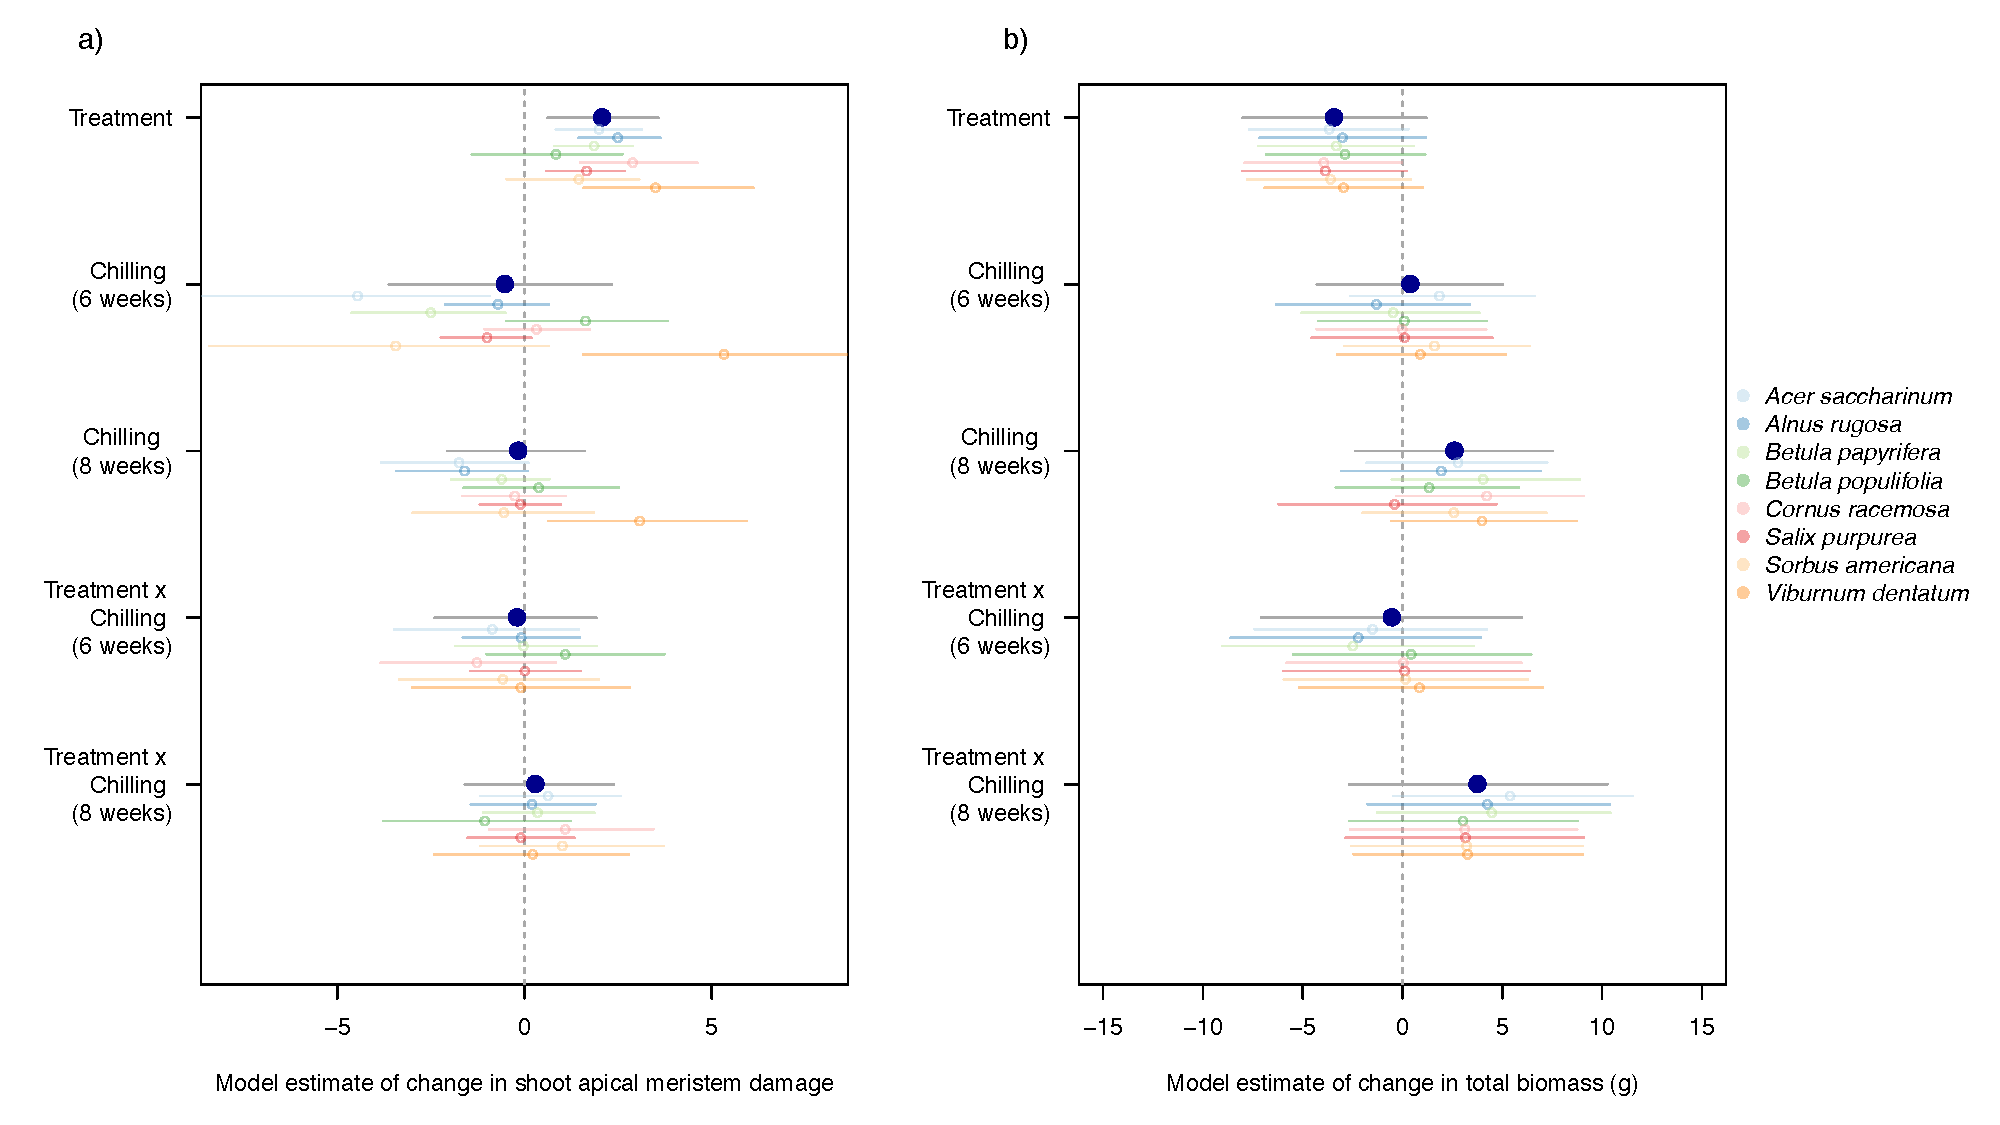
\includegraphics[width=18cm]{..//analyses/figures/mu_growth90.pdf} 
  -\caption{Effects of false spring treatment, six weeks of chilling and eight weeks of chilling on a) shoot apical meristem damage and b) total biomass. Dots and lines show means and 90\% uncertainty intervals. }\label{fig:mugrowth}
  -\end{center}
  -\end{figure}}
  
  {\begin{figure} [H]
  -\begin{center}
  -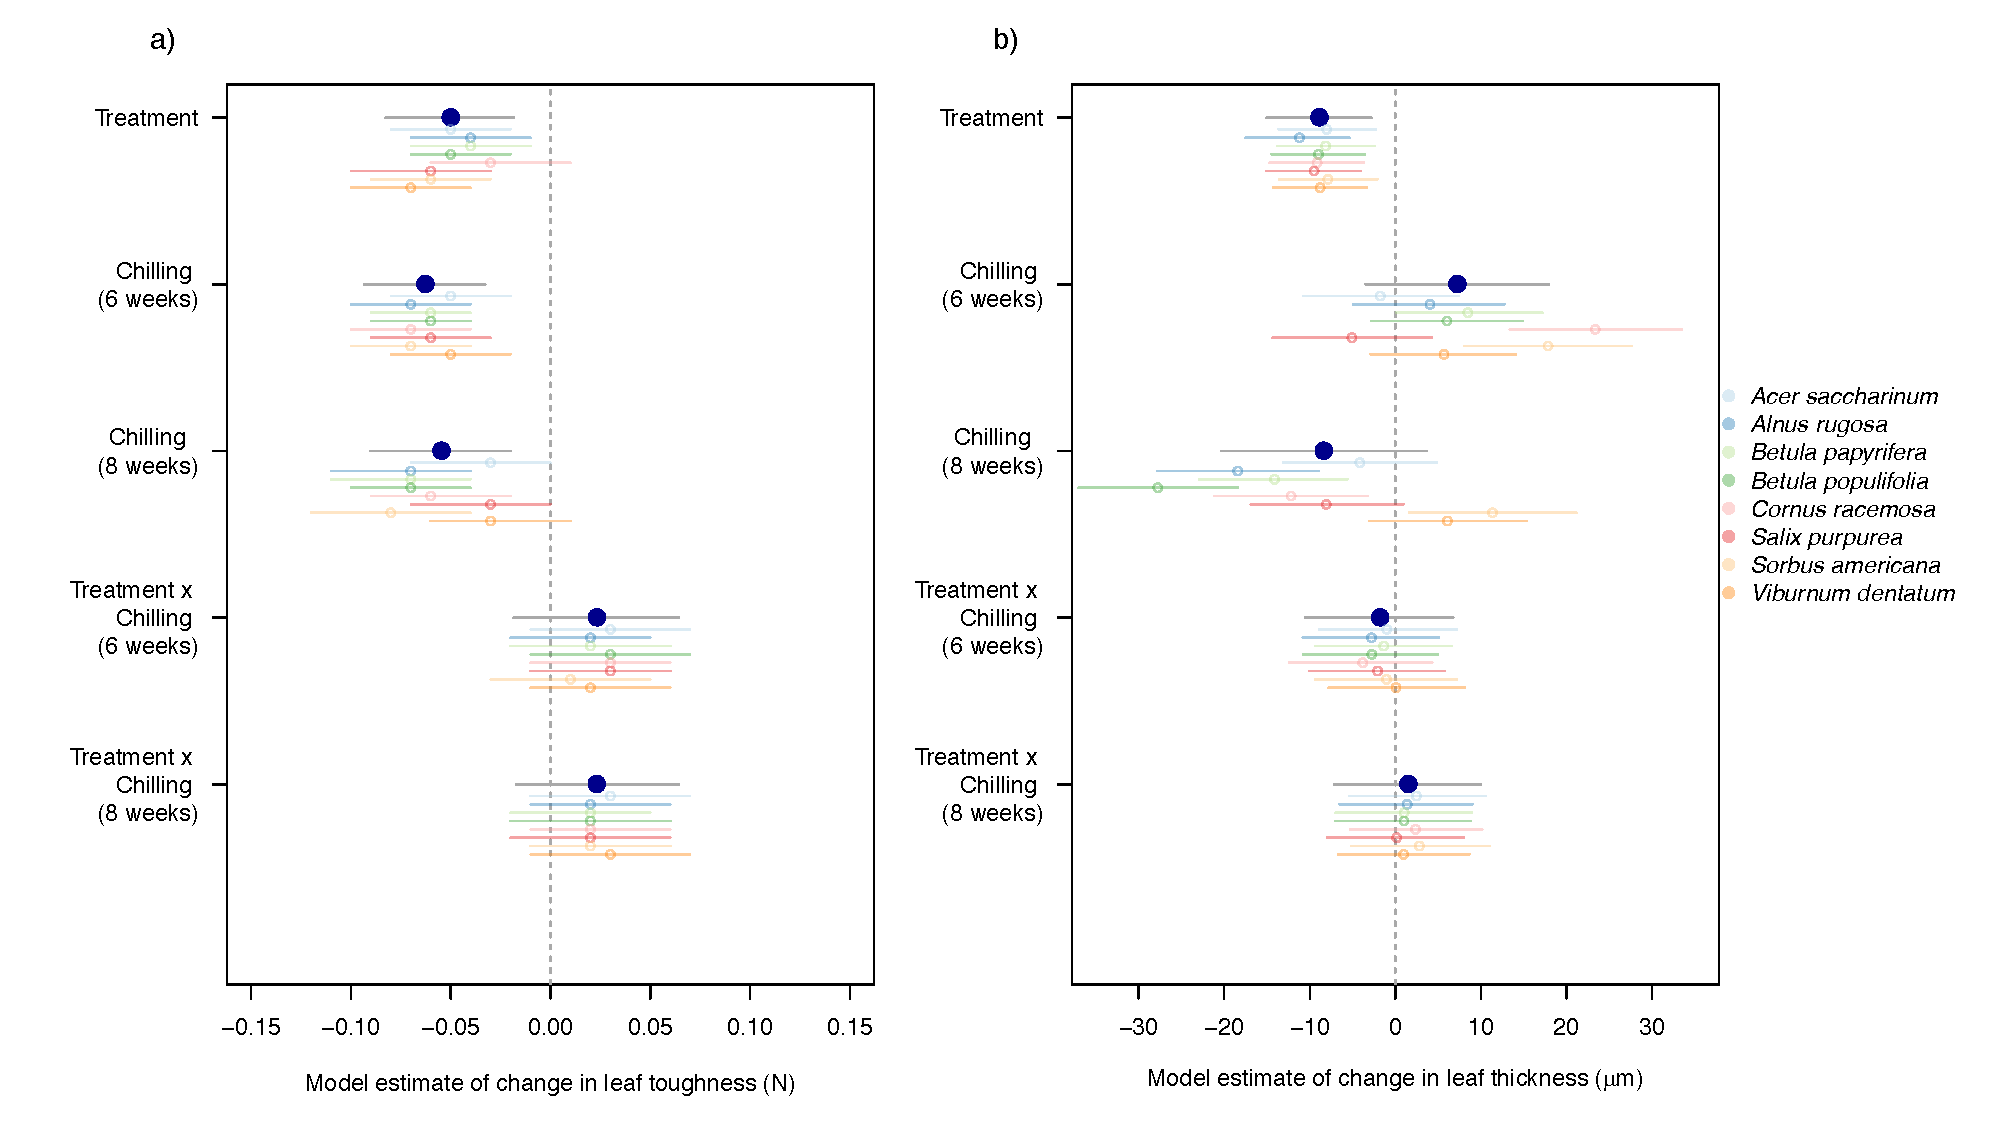
\includegraphics[width=18cm]{..//analyses/figures/mu_leaftraits90.pdf} 
  -\caption{Effects of false spring treatment, six weeks of chilling and eight weeks of chilling on a) leaf toughness and b) leaf thickness. Dots and lines show means and 90\% uncertainty intervals. }\label{fig:muleaf}
  -\end{center}
  -\end{figure}}
  

\end{document}
